\documentclass[a4paper,titlepage]{scrartcl}
\pagestyle{plain}
\usepackage[utf8]{inputenc}
\usepackage[T1]{fontenc}
\usepackage[german]{babel}
\usepackage{float}
\usepackage{graphicx,tabularx}
\usepackage{amsmath,amssymb,amstext,mathabx}
\usepackage{enumerate}
\usepackage{units,longtable}
\usepackage{mhchem, numprint,booktabs,breqn}

\renewcommand{\sc}{\textsc}
\numberwithin{equation}{section}

\title{Gitterschwingungen}
\author{Genti Saliu\\Gruppe 106}
\date{Versuchstag: 12. Januar 2015}

\begin{document}
	\begin{titlepage}
		\maketitle
		\thispagestyle{empty}
	\end{titlepage}
	
\newpage
\pagenumbering{roman}
\tableofcontents

\newpage
\pagenumbering{arabic}

\section{Ziel des Versuchs}
In diesem Versuch sollen die longitudinalen Schwingungen des Kristallgitters (Phononen) durch eine Kette aus mit Federn gekoppelten Gleitern auf einer Luftkissenbahn modelliert und die Dispersionsrelation der einatomigen und zweiatomigen Kette bestimmt werden.
\section{Theoretische Grundlagen}
\subsection{Kristallstruktur}
Kristalline Festkörper zeichnen sich durch eine räumlich periodische Anordnung der Atomgruppen aus, die durch die Begriffe \emph{Basis} und \emph{Gitter} beschrieben wird.
\begin{figure}[H]
	\centering
	\begin{tabular}{@{}r@{}}
		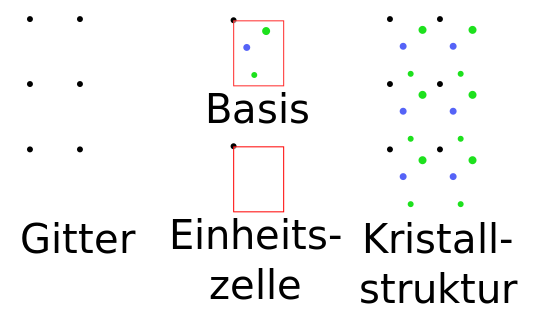
\includegraphics[width=0.5\textwidth]{kristallstruktur.png}\\
		\footnotesize\sffamily\textbf{Quelle:} Wikipedia \cite{wiki:kristallstruktur}
	\end{tabular}
	\caption{Kristallstruktur}
    \label{fig:kristallstruktur}
\end{figure}
Die \emph{Basis} einer Kristallstruktur besteht aus Atomen, Ionen oder Molekülen und stellt die kleinste Gruppe dar, die sich periodisch im dreidimensionalen Raum wiederholt. Sie besteht aus mindestens einem Atom, kann jedoch auch einige tausend Atome umfassen.\\ \\
Jeder Basis wird ein Bezugspunkt zugewiesen. Betrachtet man nur diese Punkte, so bilden sie das Kristall\emph{gitter}. Sie spannen die Basisvektoren auf, die von einem Gitterpunkt zu seinen Nachbarn weisen. Das von diesen Basisvektoren $\vec{a_i}$ aufgespannte Parallelepiped heißt Einheits- oder Elementarzelle. Diese Zelle hat an ihren Ecken je einen Gitterpunkt, muss jedoch nicht zwischen direkt benachbarten Punkten gezogen werden, sondern kann beliebig groß gewählt werden. \cite{wiki:kristallstruktur} Die Seitenlänge $a$ der Elementarzelle nennt man \emph{Gitterkonstante}.\\ \\
Die Elementarzelle mit dem kleinstmöglichen Volumen nennt man \emph{primitive Elementarzelle}. Die \emph{Wigner-Seitz-Zelle} ist eine spezielle primitive Zelle, die nur einen Gitterpunkt in ihrem Zentrum enthält und alle ihre Orte diesem Gitterpunkt näher als den benachbarten Gitterpunkten liegen. Die Wigner-Seitz-Zelle ist Ausgangspunkt zur Beschreibung vieler mechanischen und elektrischen Eigenschaften von Festkörpern. \cite{wiki:wignerseitz}\\ \\
Ein Kristall kann in sich selbst durch folgende Translation überführt werden:
\begin{equation*}
\vec{R}=\sum_{i=1}^3 n_i \vec{a_i} \quad \quad \text{mit} \quad n_i=0, \pm 1, \pm 2, ...
\end{equation*}
Das Kristallgitter, auch Punktgitter genannt, ist eine dreidimensionale Anordnung von Punkten, dessen Untereinheit die Elementarzelle ist. Diese Elementarzellen werden durch Translationssymmetrie zu einem dreidimensionalen Netz erweitert. Anhand dieser Translationssymmetrie werden Kristalle einem von 14 möglichen Bravais-Gittern eingeteilt: kubisch-primitiv, kubisch raumzentriert, kubisch flächenzentriert, tetragonal-primitiv, tetragonal-raumzentriert, orthorhombisch-primitiv, orthorhombisch-basiszentriert,\\orthorhombisch-raumzentriert, orthorhombisch-flächenzentriert und hexagonal-primitiv.\\ \\
Neben dem oben vorgestellten Punktgitter im Ortsraum definiert man ein Punktgitter im \emph{reziproken Raum}, auch genannt \emph{reziprokes Gitter}, das durch die Vektoren $\vec{b_i}$ aufgespannt wird:
\begin{equation*}
b_i=\frac{2 \pi}{V_{EZ}} a_j \times a_k
\end{equation*}
mit $V_{EZ}$ das Volumen der Einheitszelle. Der Translationsvektor im reziproken Gitter sieht dann wie folgt aus:
\begin{equation*}
\vec{G}=\sum_{i=1}^3 h_i b_i \quad \quad \text{mit} \quad h_i=0, \pm 1, \pm 2, ...
\end{equation*}
Im reziproken Gitter definiert man symmetrische Polyeder, die sogenannten Brioullin-Zonen (BZ). Die 1. BZ besteht aus allen Punkten im reziproken Raum, die dem Ursprung näher liegen als allen anderen Punkten $\vec{G}$. Die 1. BZ einer einfachen kubischen Kristallstruktur erstreckt sich in allen drei Richtungen des reziproken Raumes:
\begin{equation*}
-\frac{\pi}{a} \leq k_i \leq \frac{\pi}{a} \quad \quad \text{mit} \quad i=x,y,z
\end{equation*}
Die Wigner-Seitz-Zelle entspricht im reziproken Gitter der 1. Brioullin-Zone.
\subsection{Phasen- und Gruppengeschwindigkeit, Wellendispersion}
Eine Welle ist durch die Kreisfrequenz $\omega$ und Wellenvektor $\vec{k}$ bzw. Frequenz $\nu$ und Wellenlänge $\lambda$ charakterisiert. Der Wellenvektor steht senkrecht auf der Wellenfront der Welle und hat einen Betrag $\frac{2 \pi}{\lambda}$.\\ \\
Die Phasengeschwindigkeit $v_{ph}$ der Welle, d.h. die Geschwindigkeit mit der sich eine Phase ausbreitet, beträgt:
\begin{equation*}
v_{ph}=\frac{w}{k}=\lambda \nu
\end{equation*}
Ein Wellenpaket besitzt die Gruppengeschwindigkeit:
\begin{equation*}
v_{gr}=\frac{d \omega}{d k}
\end{equation*}
Ein Wellenpaket ist eine Welle, deren Amplitudenverlauf nur in einem begrenzten Raumgebiet ungleich Null ist. Der Amplitudenverlauf wird Hüllkurve des Wellenpakets genannt. Das Wellenpaket kann als Überlagerung von Einzelwellen mit verschiedenen Frequenzen vorgestellt werden, die sich mit einer bestimmten Phasengeschwindigkeit ausbreiten, die frequenzabhängig sein kann. Die Hüllkurve bewegt sich jedoch mit Gruppengeschwindigkeit. \cite{wiki:gruppengeschwindigkeit}\\ \\
Im einfachen Fall der elektromagnetischen Welle im Vakuum mit $w=ck$ fallen Phasen- und Gruppengeschwindigkeit zusammen und sind gleich der Proportionalitätskonstante $c$.\\ \\
Propagiert die Welle jedoch durch Materie, so hebt sich die Linearität zwischen $\omega$ und \textbf{k} auf. Die Folge ist das Auftreten von Dispersion: Phasen- und Gruppengeschwindigkeit werden abhängig von der Frequenz bzw. von der Wellenlänge und fallen nicht mehr zusammen. Dispersion bezeichnet man die Abhängigkeit einer Größe von der Frequenz. In der Regel ist die Ohasengeschwindigkeit größer als die Gruppengeschwindigkeit ($v_{ph}>v_{gr}$).\\ \\
Die Funktion $w=f(k)$ nennt man Dispersionsrelation oder Dispersionsbeziehung. Aus deren Steigung lässt sich die Gruppengeschwindigkeit bestimmen.
\subsection{Stehende Wellen}
Eine stehende Welle ist eine Welle, deren Auslenkung an bestimmten Stellen immer Null bleibt, ihre Gruppengeschwindigkeit ist $v_{gr}=0$. Sie entsteht als Überlagerung zweier gegenläufig fortschreitender Wellen gleicher Frequenz und Amplitude, die aus verschiedenen Erregern stammen oder durch Reflexion einer Welle an einem Hindernis entstehen. \cite{wiki:stehendewelle}\\ \\
Im Folgenden untersuchen wir die Wellen für Systeme mit kontinuierlichen und diskontinuierlichen, diskreten Masenverteilungen.
\subsubsection{Kontinuierliche Massenverteilung}
Betrachtet man einen zwischen festen Enden im Abstand $L$ eingespannten, eindimensionalen Strang mit kontinuierlichen, homogenen Massenverteilung, so führt diese Randbedingung zur Ausbildung stehenden Wellen:
\begin{equation}
\label{eq:stehendeWelleKontinuierlich}
L=n \cdot \frac{\lambda}{2} \quad \quad \text{mit} \quad n=1,2,...
\end{equation}
Damit sind nur Wellenlängen $\lambda_n=\frac{2L}{n}$ möglich. Die entsprechenden Wellenvektoren sind:
\begin{equation*}
k_n=\frac{2 \pi}{\lambda_n}=\frac{n \pi}{L}
\end{equation*}
Die zugehörige Frequenz $\omega_n$ heißt Eigenfrequenz, $n$ heißt Modenzahl und man spricht von der $n.$ Eigenschwingung, Mode oder Eigenmode.\\ \\
Im Fall eines unendlich dünnen Strangs ist die Zahl der Eigenfrequenzen unbegrenzt.
\subsubsection{Diskontinuierliche, diskrete Massenverteilung}
Wir nehmen die Masse des eindimensionalen Strangs als diskrete gleiche Punktmassen mit einen zunächst festen Abstand $a$ voneinander an. Die Punktmassen sind jeweils über Federn mit ihren Nachbarn gekoppelt. Sei Abstand $a$ der sich von selbst einstellende Gleichgewichtsabstand. Die Massen können aufgrund der Kopplung um diese Gleichgewichtspositionen schwingen. Diese Miteinanderkopplung von Massenpunkten nennt man \emph{lineare Kette}.\\ \\
Bei festen Enden sind wieder nur stehende Wellen möglich. Die Auslenkung ist jedoch nur an den Stellen der Massenpunkte definiert, denn dazwischen existiert keine Materie. Die Wellenlänge ist somit nicht eindeutig bestimmbar, denn zu jeder möglichen Welle mit $\lambda < 2a$ eine langwellige Welle mit $\lambda > 2a$ existiert, die ein identisches Auslenkungsmuster der Punktmassen besitzt (s. Abbildung \ref{fig:diskreteStehendeWelle}).
\begin{figure}[H]
	\centering
	\begin{tabular}{@{}r@{}}
		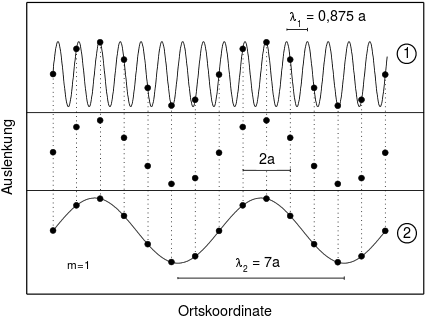
\includegraphics[width=0.5\textwidth]{stehendewellediskret.png}\\
		\footnotesize\sffamily\textbf{Quelle:} Vorbereitungsmappe \cite{vorbereitungsmappe}
	\end{tabular}
	\caption{Auslenkungsmuster des eindimensionalen Punktmassegitters}
    \label{fig:diskreteStehendeWelle}
\end{figure}
Die unterschiedlichen Wellen mit gleicher Auslenkung sind also physikalisch nicht unterscheidbar. Um diesen Zustand zu beschreiben, genügt es vollständig, sich auf eine Welle zu beschränken. Wir wählen diejenige mit $\lambda > 2a$, da hier nur eine passende Welle für ein bestimmmtes Auslenkungsmuster existiert, während es im kurzwelligen Bereich $\lambda < 2a$ unendlich viele sind. Somit gilt:
\begin{align*}
\lambda_{min}&=2a\\
\lambda_{max}&=2L
\end{align*}
Aus \ref{eq:stehendeWelleKontinuierlich} folgt die maximale Modenzahl $n_{max}$:
\begin{equation*}
n_{max}=\frac{2L}{\lambda_{min}}=\frac{L}{a}
\end{equation*}
Der maximale Wellenvektor ergibt sich zu:
\begin{equation*}
k_{max}=\frac{2 \pi}{\lambda_{min}}=\frac{\pi}{a}
\end{equation*}
\subsection{Gitterschwingungen: eindimensionales Modell für ein Gitter realer Atome}
Damit ein reales Atomgitter auf eine lineare Kette von Punktmassen abgebildet werden kann, muss, zum Einen, die Wechselwirkung zwischen den Atomen des Gitters bekannt sein, zum Anderen muss geklärt werden, ob Atome als Punktmassen behandelt werden können.\\ \\
In einem Atomgitter können die Atome als Punktmassen behandelt werden, denn die Masse des Atoms ist überwiegend im Kern konzentriert und der Kernradius ist viel kleiner als der Gitterabstand.\\ \\
Die Wechselwirkung zwischen Atomen findet durch den Überlapp der Wellenfunktionen der Elektronen der äußeren Schale statt. Die inneren Schalen und den Kern bezeichnet man als Atomrumpf. Die Gesamtenergie des Systems aus Valenzelektronen und positiven Atomrümpfen besitzt ein Minimum bei einem bestimmten Atomkernabstand $x_0$. Das ist der Gleichgewichtsabstand und entspricht der Bindungslänge. Wird der Atom aus der Minimumslage ausgelenkt, so erhöht sich die Energie der Valenzelektronen. Da diese Energieerhöhung zu klein ist, um höhere Zustände anzuregen, wird diese Energie beim Rückgang der Auslenkung wieder zurückgewonnen. Der Atomrumpf schwingt daher reibungsfrei im Potenzial der Valenzelektronen. Der Verlauf dieses Potenzials ist in Abbildung \ref{fig:gitterschwingung} dargestellt.
\begin{figure}[H]
	\centering
	\begin{tabular}{@{}r@{}}
		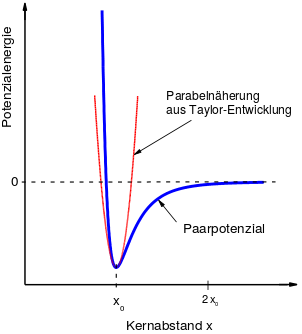
\includegraphics[width=0.4\textwidth]{gitterschwingung.png}\\
		\footnotesize\sffamily\textbf{Quelle:} Vorbereitungsmappe \cite{vorbereitungsmappe}
	\end{tabular}
	\caption{Paarpotenzial zwischen 2 Atomen als Funktion des Kernabstands}
    \label{fig:gitterschwingung}
\end{figure}
Für kleine Auslenkungen aus der Gleichgewichtslage (s. Abbildung \ref{fig:gitterschwingung}) kann dieses Potenzial durch eine Taylorentwicklung bis zur 2. Ordnung genährt (harmonische Näherung) werden:
\begin{equation*}
\Phi(x)=\Phi_0+\frac{1}{2} \frac{\partial^2 \Phi}{\partial x^2}\bigg|_{x_0} (x-x_0)^2
\end{equation*}
Desweiteren führen wir noch die Näherung der sogenannten Nächste-Nachbar-Wechselwirkung, wo nur die Wechselwirkung mit direkten Nachbarn berücksichtigt wird und die mit entfernten Atomen vernachlässigt wird. Es wirken also auf ein Atom nur Kräfte der jeweils rechten und linken Nachbarn.\\ \\
Mit diesen Näherungen reduzieren sich die Kräfte auf die Punktmasse aufgrund der harmonischen Kopplung auf zwei Hookesche Federkräfte. Der Term $\frac{\partial^2 \Phi}{\partial x^2}\bigg|_{x_0}$ entspricht der Federkonstante $D$ der Hookeschen Kraft $F=-Dx$.
\subsubsection{Einatomige Kette}
Die lineare einatomige Kette räpresentiert ein eindimensionales Atomgitter mit Gitterabstand $a$ und einem Atom der Masse $m$ in der Basis. Sie besteht aus Punktemassen der Masse $m$ mit Ruheabstand $a$, verbunden durch masselose Hookesche Federn mit Federkonstante $D$ (s. Abbildung \ref{fig:einatomkette}).
\begin{figure}[H]
	\centering
	\begin{tabular}{@{}r@{}}
		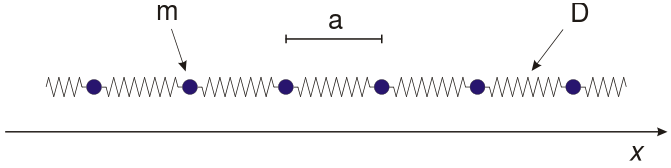
\includegraphics[width=0.7\textwidth]{einatomkette.png}\\
		\footnotesize\sffamily\textbf{Quelle:} Vorbereitungsmappe \cite{vorbereitungsmappe}
	\end{tabular}
	\caption{Lineare einatomige Kette}
    \label{fig:einatomkette}
\end{figure}
Wir wollen nun die Dispersionsrelation der einatomigen Kette bestimmen. Dazu betrachten wir die Newtonsche Bewegungsgleichung für einen Massenpunkt:
\begin{equation*}
m\ddot{s_j}(t)=F_{j,j+1}+F_{j,j-1}
\end{equation*}
Dabei ist $F_{j,j+1}$ die Kraft auf den Massenpunkt $j$ durch die rechte Feder und $F_{j,j-1}$ die Kraft auf den Massenpunkt $j$ durch die linke Feder.
\begin{figure}[H]
	\centering
	\begin{tabular}{@{}r@{}}
		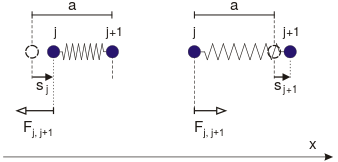
\includegraphics[width=0.5\textwidth]{einatomkettekraft.png}\\
		\footnotesize\sffamily\textbf{Quelle:} Vorbereitungsmappe \cite{vorbereitungsmappe}
	\end{tabular}
	\caption{Änderung der Federlänge}
    \label{fig:einatomkettekraft}
\end{figure}
Wie man der Abbildung \ref{fig:einatomkettekraft} entnehmen kann, lassen sich die Kräfte $F_{j,j+1}$ und $F_{j,j-1}$ bestimmen zu:
\begin{align*}
F_{j,j+1}&=-D \cdot s_j + D \cdot s_{j+1}=-D \cdot (s_j + s_{j + 1})\\
F_{j,j-1}&=-D \cdot s_j + D \cdot s_{j-1}=-D \cdot (s_j - s_{j - 1})
\end{align*}
Nach Einsetzen der Kräfte schreibt sich die Netwonsche Bewegungsgleichung zu:
\begin{equation*}
m\ddot{s_j}(t)=D(s_{j+1} + s_{j-1} - 2 s_j)
\end{equation*}
Die obige DGL lässt sich mit dem Ansatz $s_j=s_0 \cdot e^{i(kx-\omega t)}$ lösen. Da die Auslenkungen $x$ nur an den diskreten Gitterpunkten $x_{0,j}$ definiert sind, lässt sich $x$ als Vielfaches des Gitterabstands $a$ schreiben mit $x_{0,j}=a \cdot j$. Wir erhalten:
\begin{equation*}
m \omega^2=D(2-(e^{ika}+e^{-ika}))=D(2-2 \cdot \cos{(ka)}
\end{equation*}
Durch Umformen und Einsetzen der trigonometrischen Identität $1-\cos{(x)}=2\sin^2{(\frac{x}{2})}$ erhalten wir die Dispersionsrelation der linearen einatomigen Kette:
\begin{equation}
\omega(k)=\sqrt{\frac{4D}{m}}\bigg|\sin{\left(\frac{ka}{2}\right)}\bigg|
\label{eq:dispersionsrelationeinatom}
\end{equation}
Abbildung \ref{fig:einatomkettedispersion} veranschaulicht die Dispersionsrelation.
\begin{figure}[H]
	\centering
	\begin{tabular}{@{}r@{}}
		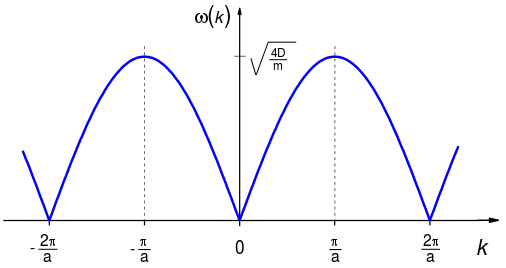
\includegraphics[width=0.5\textwidth]{einatomkettedispersion.png}\\
		\footnotesize\sffamily\textbf{Quelle:} Vorbereitungsmappe \cite{vorbereitungsmappe}
	\end{tabular}
	\caption{Dispersionsrelation der linearen einatomigen Kette}
    \label{fig:einatomkettedispersion}
\end{figure}
Die $k$-Werte können aus den Bedingungen der stehenden Welle bestimmt werden. Da bei einem Kristall die Zahl der Atome sehr groß ist, zeigt die Dispersionskurve einen kontinuierlichen Verlauf. Der Modellkristall unseres Versuchs besitzt nur  12 Massen, sodass die Kurve in diesem Fall auch nur aus 12 Punkten besteht.\\ \\
\textbf{Grenzfälle für kleine und große k}
\begin{description}
  \item[$k \rightarrow 0$ (Zonenzentrum)] Für kleine $k$ oder lange Wellen (große $\lambda$) können wir die Kleinwinkelnäherung der Sinusfunktion ($\sin{(x)} \approx x$) anwenden. Die Dispersionsrelation beträgt:
  \begin{equation}
  \omega(k)=\sqrt{\frac{4D}{m}} \cdot \bigg|\frac{ka}{2}\bigg|=\sqrt{\frac{Da^2}{m}}|k|
  \label{eq:einatomDispersionsrelationLangeW}
  \end{equation}
  Die Phasen- und Gruppengeschwindigkeiten fallen zusammen, die Wellenausbreitung wird dispersionsfrei:
  \begin{equation}
  v_{gr}=v_{ph}=\frac{\omega}{k}=\frac{d \omega}{dk}=\sqrt{\frac{Da^2}{m}}
  \label{eq:einatomSchallgeschwindigkeit}
  \end{equation}
  Diese Geschwindigkeit entspricht der Schallgeschwindigkeit der linearen Kette und ist die größte in einem Kristall auftretende Wellenausbreitungsgeschwindigkeit.
  \item[$k \rightarrow \frac{\pi}{a}$ (Zonenrand)] Die Steigung der Dispersionskurve geht gegen Null, für $k=\frac{\pi}{a}$ gilt $v_{gr}=0$. Die Wellenlänge wird mit $\lambda=2a$ minimal.
\end{description}
\textbf{Schwingungsmoden des Modellkristalls}\\
Die stehende Welle in unserem Modellkristall entsteht aus einer einlaufenden und einer zurücklaufenden Welle mit Phasenverschiebung $\pi$:
\begin{equation*}
s_j=2s_0 \cdot \sin{(\omega t)} \cdot \sin{(k_n a_1 \cdot j)}
\end{equation*}
wobei $a_1$ für die Gitterkonstante der einatomigen Kette steht. Im Modellkristall mit 12 Massen ist die Länge $L$ durch $12+1$ Federlängen bzw. Gitterkonstanten gegeben. Daher ist $L=13a_1 \label{eq:einatommodell}$ und es gilt:
\begin{equation*}
k_n=\frac{n \pi}{L}=\frac{n \pi}{13 a_1}
\end{equation*}
Die maximale Anzahl der Moden entspricht der Anzahl der Massen: $n_{max}=12$. Die stehende Welle ist proportional zu $\sin{\left(\frac{n \pi}{13} j\right)}$ mit $j=1,...,12$.
\subsubsection{Zweiatomige Kette}
Die lineare zweiatomige Kette repräsentiert ein eindimensionales Atomgitter mit Gitterabstand $a$ und zwei Atomen pro Basis, die unterschiedliche Massen haben. Das leichtere Atom besitzt eine Masse $m$, das schwerere eine Masse $M$. Sie besteht aus Punktmassen, die durch ideale Hookesche Federn im Abstand $\frac{a}{2}$ verbunden sind und abwechselnd die Massen $m$ und $M$ haben (Abbildung \ref{fig:zweiatomkette}).
\begin{figure}[H]
	\centering
	\begin{tabular}{@{}r@{}}
		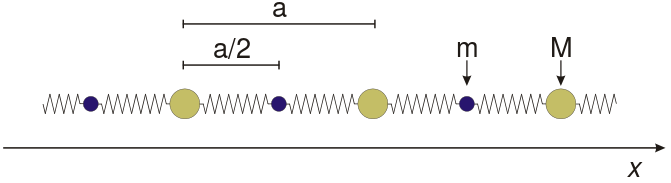
\includegraphics[width=0.7\textwidth]{zweiatomkette.png}\\
		\footnotesize\sffamily\textbf{Quelle:} Vorbereitungsmappe \cite{vorbereitungsmappe}
	\end{tabular}
	\caption{Lineare zweiatomige Kette}
    \label{fig:zweiatomkette}
\end{figure}
Analog zur einatomigen Kette bestimmen wir die Dispersionsrelation aus den gekoppelten Newtonschen Bewegungsgleichungen (s. Abbildung \ref{fig:zweiatomkettekraft}):
\begin{align*}
m \ddot{s}_j&=D(s_{j+1} + s_{j-1} - 2s_j)\\
M \ddot{s}_{j+1}&=D(s_{j+2} + s_j - 2s_{j+1})
\end{align*}
\begin{figure}[H]
	\centering
	\begin{tabular}{@{}r@{}}
		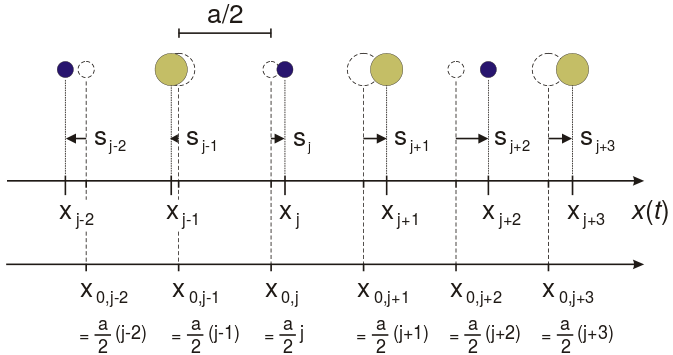
\includegraphics[width=0.7\textwidth]{zweiatomkettekraft.png}\\
		\footnotesize\sffamily\textbf{Quelle:} Vorbereitungsmappe \cite{vorbereitungsmappe}
	\end{tabular}
	\caption{Auslenkungen in der linearen zweiatomigen Kette}
    \label{fig:zweiatomkettekraft}
\end{figure}
Die DGLs lösen sich mit den folgenden Ansätzen:
\begin{align*}
s_j&=s_{0,m} \cdot e^{i(ka - \omega t)}\\
s_{j+1}&=s_{0,M} \cdot e^{i(ka - \omega t)}
\end{align*}
Wir erhalten das Gleichungssystem:
\begin{align*}
- \omega^2 m s_{0,m}&=D s_{0,M}(1+e^{-ika})-2D s_{0,m}\\
- \omega^2 M s_{0,M}&=D s_{0,m}(1+e^{ika})-2D s_{0,M}
\end{align*}
Über die Forderung der Existenz einer nichttrivialen Lösung des linearen Gleichungssystems erhalten wir die Dispersionsrelation:
\begin{equation}
\omega^2_{\pm}=D \left(\frac{1}{m} + \frac{1}{M}\right) \pm D \sqrt{\left(\frac{1}{m} + \frac{1}{M}\right)^2-\frac{4}{m M} \sin^2{\left(\frac{ka}{2}\right)}}
\label{eq:dispersionsrelationzweiatom}
\end{equation}
Abbildung \ref{fig:zweiatomkettedispersion} zeigt diese Dispersionsrelation. Es fällt auf, dass es zwei unterschiedliche Lösungen der Dispersionsrelation existieren, die jeweils akustischer ($\omega_{-}$) und optischer ($\omega_{+}$) Zweig genannt sind und durch eine Frequenzlücke getrennt sind.
\begin{figure}[H]
	\centering
	\begin{tabular}{@{}r@{}}
		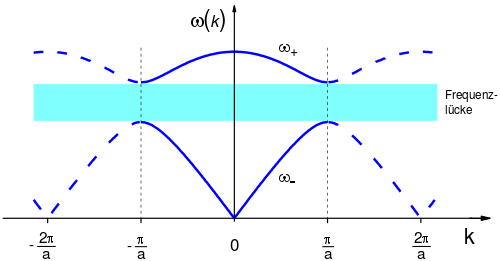
\includegraphics[width=0.7\textwidth]{zweiatomkettedispersion.png}\\
		\footnotesize\sffamily\textbf{Quelle:} Vorbereitungsmappe \cite{vorbereitungsmappe}
	\end{tabular}
	\caption{Dispersionsrelation der linearen zweiatomigen Kette}
    \label{fig:zweiatomkettedispersion}
\end{figure}
Die Dispersionsrelation ist periodisch mit Periode $\frac{2 \pi}{a}$.\\ \\
Der $\omega_{+}$-Ast heißt optischer Ast, weil die leichten und schweren Massen gegeneinander schwingen, sodass bei unterschiedlicher elektrischer Ladung die Atome $m$ und $M$ einen schwingenden Dipol bilden. Der Dipol kann elektromagnetische Strahlung absorbieren oder emittieren, die Schwingung wird ''optisch aktiv''. Die unterschiedliche Ladung resultiert aus dem ionischen oder polaren Charakter der chemischen Bindung in Kristallen.\\ \\
Der $\omega_{-}$-Ast heißt ''akustischer Ast'', da er für $k \rightarrow 0$ die größte Gruppengeschwindigkeit innerhalb der Kette aufweist, d.h. die akustische Schallgeschwindigkeit $v_s$.\\ \\
Der Frequenzbereich zwischen den Ästen wird nie überstrichen, deshalb existiert im Frequenzspektrum der Schwingungsmoden eine Frequenzlücke.\\ \\
\textbf{Grenzfälle}
\begin{description}
\item[$k \rightarrow 0$ (Zonenzentrum)] Man kann wieder die Kleinwinkelnäherung der Sinusfunktion anwenden und man erhält folgende Dispersionsrelationen:
\begin{align*}
\omega_{-}(k)&=\sqrt{\frac{Da^2}{2(m+M)}k}\\
\omega_{+}(k)&=\sqrt{2D \left(\frac{1}{m} + \frac{1}{M}\right)}
\end{align*}
Aus dem akustischen Ast erhalten wir die Gruppen- und Phasengeschwindigkeiten:
\begin{equation}
v_{gr}=\frac{d \omega}{dk}=v_{ph}=\frac{\omega(k)}{k}=\sqrt{\frac{Da^2}{2(m+M)}}
\label{eq:zweiatomschallgeschwindigkeit}
\end{equation}
\item[$k \rightarrow \frac{\pi}{a}$ (Zonenrand)] Die Dispersionsrelationen werden zu:
\begin{align*}
\omega_{+}^2=\frac{2D}{m}\\
\omega_{-}^2=\frac{2D}{m}
\end{align*}
\end{description}
\textbf{Modellkristall}\\
Der Modellkristall für die zweiatomige Kette ist fast gleich wie der der einatomigen Kette. Es wurden nur zuzätzliche Gewichte auf jedem zweiten Gleiter gelegt und es gibt wieder 13 Federlängen, jedoch erstreckt sich die Gitterkonstante $a_2$ über 2 Federn. Die Länge ist somit $L=6.5 \cdot a \label{eq:zweiatommodell}$ und es gilt:
\begin{align*}
k_n&=\frac{n \pi}{6.5 a_2}\\
n_{max}&=6
\end{align*}
\section{Experimenteller Aufbau}
Die linearen Ketten werden durch eine Anordnung von 12 durchnummerierten Massengleitern realisiert, die mit Federn gleicher Federkonstante $D$ miteinander verbunden sind und zur Reibungsminimierung sich auf eine Luftkissenbahn bewegen.\\ \\
Die Gleiter werden um $\unit[1]{mm}$ durch eine Turbine hochgehoben, die Luft in die Luftkissenbahn drückt.\\ \\
Die periodische Anregung der Kette erfolgt mit einem Schrittmotor, der eine harmonische Bewegung mit variabler Anregungsamplitude erlaubt. Die Anregungsfrequenz kann auf Werten zwischen $\unit[0.1526]{Hz}$ bis $\unit[2.846]{Hz}$ eingestellt werden.\\ \\
Die Gleiter sind mit Reflektoren ausgestattet, die die von den LEDs der ''VideoCom''-Kamera periodisch abgegebenen Lichtblitze reflektieren und durch das Objektiv der Kamera auf eine CCD-Zeile abgebildet werden. Die Wiederholzeit der Lichtblitze kann zwischen $\unit[200]{ms}$ und $\unit[6.25]{s}$ variiert werden, für den Versuch beträgt sie jedoch $\unit[25]{ms}$. Die CCD-Zeile wird mit der gleichen Wiederholzeit ausgelesen und dabei die Pixelpositionen an das Programm ''Gitterschwingungen'' übergeben, das dann aus den Auslenkungen $x(t)$ die Eigenfrequenzen mithilfe einer schnellen Fourier-Transformation berechnet und in $\unit[]{Hz}$ anzeigt.\\ \\
Die Kamera muss so positioniert werden, dass sie 2 benachbarte Gleiter mit nicht abgedeckten Reflektoren sieht. Die Reflektoren der anderen Gleiter sollen abgedeckt sein, damit sie von der Kamera nicht detektiert werden. Ausserdem soll man die Kamera justieren, um die 2 Gleiterstriche in der CCD-Zeile richtig abbilden zu können.\\ \\
Zur Simulation der zweiatomigen Kette werden einige Gleiter mit einem zusätzlichen Gewicht versehen.
\section{Durchführung des Versuchs}
Bevor wir mit den Messungen angefangen haben, wurden wir durch den Betreuer in die Bedienung der verschiedenen Versuchgeräte eingewiesen. Wir starteten die Turbine der Luftkissenbahn, brachten die Auslenkung des Schrittmotors in Nulllage, schalteten die ''VideoCom''-Kamera, den Computer und die Hilfprogramme ein.\\ \\
Wir stellten sicher, dass nur 2 Gleiter für die ''VideoCom''-Kamera sichtar waren. Die Kamera war bereits korrekt positioniert und justiert, sodass wir keine Einstellungen vornehmen mussten. Die fokussierten Gleiter waren die mit den Nummern 5 und 6.
\subsection{Eigenfrequenzen der einatomigen und zweiatomigen Kette}
In diesem Versuch messten wir die Eigenfrequenzen der einatomigen und zweiatomigen Kette.\\ \\
Wir haben mit der einatomigen Kette angefangen. Wir nahmen die Eigenfrequenzen mithilfe des LabVIEW-Programms ''Gitterschwingungen'' in 4 Datensätzen mit einer Dauer von $\unit[100]{s}$ auf. Vor jeder Aufnahme regten wir unterschiedliche Gleiter (Nummer 9, 6 und 3) mit einem kurzen Stoß per Hand zur Auslenkung an, nachdem die vorherigen Schwingungen der Kette durch mehrmaliges Zuhalten der Turbinenansaugangsöffnung zur Ruhe gebracht wurden. Die Messwerte sind in Tabelle \ref{tab:eigenfreqEinatom} aufgeführt.\\ \\
Danach wurden die Eigenfrequenzen der zweiatomigen Kette gemessen. Die zweiatomige Kette mit 2 verscheidenen Massen wurde realisiert, indem man jeden zweiten Gleiter mit einem Zusatzgewicht versehen hat. Es galt das gleiche Messprinzip wie für die einatomige Kette, wobei wir hier die Gleiter mit den Nummern 3, 6, 8 und 12 per Hand anregten. Die Messergebnisse entnehmen Sie der Tabelle \ref{tab:eigenfreqZweiatom}.
\begin{table}[H]
\centering
\tabcolsep=0.11cm
\begin{tabular}{ccccccccc}
\toprule
& \multicolumn{2}{c}{1. Datensatz} & \multicolumn{2}{c}{2. Datensatz} & \multicolumn{2}{c}{3. Datensatz} & \multicolumn{2}{c}{4. Datensatz}\\
\cmidrule(r){2-3} \cmidrule(r){4-5} \cmidrule(r){6-7} \cmidrule(r){8-9}
Mode & Gleiter 5 & Gleiter 6 & Gleiter 5 & Gleiter 6 & Gleiter 5 & Gleiter 6 & Gleiter 5 & Gleiter 6\\
\hline
1 & 0.276800 & 0.276803 & 0.277464 & 0.277463 & 0.276940 & 0.276939 & 0.276124 & 0.276126\\
2 & 0.551400 & 0.551400 & 0.550223 & 0.550246 & 0.551431 & 0.551428 & 0.550315 & 0.550318\\
3 & 0.817257 & 0.817254 & 0.816051 & 0.816035 & 0.817573 & 0.817572 & 0.817583 & 0.817561\\
4 & 1.073536 & 1.073084 & 1.073320 & 1.073253 & 1.073703 & 1.073683 & 1.072351 & 1.072154\\
5 & 1.313072 & 1.313113 & 1.314681 & 1.314679 & 1.314338 & 1.314344 & 1.314130 & 1.314140\\
6 & 1.535535 & 1.535524 & 1.536911 & 1.536889 & 1.537003 & 1.537010 & 1.535691 & 1.535629\\
7 & 1.739765 & 1.739774 & 1.740109 & 1.740094 & 1.740200 & 1.740164 & 1.740231 & 1.740202\\
8 & 1.917841 & 1.917969 & 1.918998 & 1.919140 & 1.917661 & 1.917741 & 1.918203 & 1.918263\\
9 & 2.067239 & 2.067344 & 2.067598 & 2.067945 & 2.067159 & 2.067117 & 2.067813 & 2.067824\\
10 & 2.187740 & 2.187746 & 2.187243 & 2.187544 & 2.187892 & 2.187883 & 2.188963 & 2.189127\\
11 & 2.277282 & 2.277294 & 2.276659 & 2.276642 & 2.275749 & 2.275110 & 2.276467 & 2.276799\\
12 & 2.327841 & 2.327748 & 2.328197 & 2.328106 & 2.328892 & 2.328834 & 2.328007 & 2.328006\\
\bottomrule
\end{tabular}
\caption{Eigenfrequenzen der einatomigen Kette in $\unit[]{Hz}$}
\label{tab:eigenfreqEinatom}
\end{table}
\begin{table}[H]
\centering
\tabcolsep=0.11cm
\begin{tabular}{ccccccccc}
\toprule
& \multicolumn{2}{c}{1. Datensatz} & \multicolumn{2}{c}{2. Datensatz} & \multicolumn{2}{c}{3. Datensatz} & \multicolumn{2}{c}{4. Datensatz}\\
\cmidrule(r){2-3} \cmidrule(r){4-5} \cmidrule(r){6-7} \cmidrule(r){8-9}
Mode & Gleiter 5 & Gleiter 6 & Gleiter 5 & Gleiter 6 & Gleiter 5 & Gleiter 6 & Gleiter 5 & Gleiter 6\\
\hline
1 & 0.240063 & 0.240064 & 0.240981 & 0.240981 & 0.239820 & 0.239817 & 0.240050 & 0.240052\\
2 & 0.477028 & 0.477025 & 0.476105 & 0.475868 & 0.476495 & 0.476601 & 0.476542 & 0.476552\\
3 & 0.704877 & 0.704884 & 0.704649 & 0.704658 & 0.705470 & 0.705475 & 0.705657 & 0.705654\\
4 & 0.919016 & 0.919079 & 0.919108 & 0.919054 & 0.918922 & 0.918935 & 0.919194 & 0.919178\\
5 & 1.110584 & 1.110585 & 1.111413 & 1.1111432 & 1.111496 & 1.111451 & 1.111731 & 1.111725\\
6 & 1.248375 & 1.248426 & 1.248730 & 1.248589 & 1.249158 & 1.249167 & 1.249751 & 1.249742\\
7 & 1.659992 & 1.659906 & 1.660968 & 1.660972 & 1.660559 & 1.660546 & 1.660895 & 1.660699\\
8 & 1.757790 & 1.757519 & 1.757680 & 1.757559 & 1.756624 & 1.756412 & 1.757384 & 1.757648\\
9 & 1.867276 & 1.867134 & 1.866565 & 1.866757 & 1.867893 & 1.867894 & 1.867410 & 1.867424\\
10 & 1.964549 & 1.964561 & 1.965178 & 1.965187 & 1.964879 & 1.964887 & 1.965090 & 1.965146\\
11 & 2.035767 & 2.035682 & 2.035868 & 2.036438 & 2.036601 & 2.036744 & 2.035461 & 2.035746\\
12 & 2.078601 & 2.078571 & 2.079307 & 2.079331 & 2.079370 & 2.079415 & 2.079656 & 2.079787\\
\bottomrule
\end{tabular}
\caption{Eigenfrequenzen der zweiatomigen Kette in $\unit[]{Hz}$}
\label{tab:eigenfreqZweiatom}
\end{table}
\subsection{Amplitudenverhältnis}
In diesem Versuchsteil sollten die Amplitudenverhältnisse der leichten und schweren Gleiter für die 6 optischen und 6 akustischen Moden der zweiatomigen Kette bestimmt werden.\\ \\
Diese Moden werden durch einen Schrittmotor angeregt, indem man die für die zweiatomige Kette gemessenen Eigenfrequenzen $f$ aus Tabelle \ref{tab:eigenfreqZweiatom} mittelt und die jeweiligen Periodendauern am Schrittmotor nach den Tabellen \ref{tab:akustisch} und \ref{tab:optisch} einstellt. Welche Eigenfrequenzen welcher Mode gehören, lässt sich aus dem Wellenvektor $k_n$ mit der im Abschnitt \ref{subsec:gesamtlaenge} gemessenen Länge bestimmen, die Einordnung in akustischem Ast bzw. optischem Ast erfolgt durch Vergleich der Beiträge der Kreisfrequenzen $\omega_n$ im Sinne von Abbildung \ref{fig:zweiatomkettedispersion}.
\begin{table}[H]
\centering
\begin{tabular}{c||c|c||c|c}
Mode $n$ & $\overline{f}$ $[\unit[Hz]]$ & $T=\frac{1}{\overline{f}}$ [\unit[]{s}] & $k_n=\frac{n \pi}{L}$ $[\unit[]{m^{-1}}]$ & $\overline{\omega}_n=2 \pi \overline{f}$ $[\unit[]{Hz}]$\\
\hline
1 & 0.240229 & 4.162700 & 0.578562 & 1.509400\\
2 & 0.476527 & 2.098520 & 1.157120 & 2.994110\\
3 & 0.705166 & 1.418110 & 1.735690 & 4.430690\\
4 & 0.919061 & 1.088070 & 2.314250 & 5.774630\\
5 & 1.111270 & 0.899875 & 2.892810 & 6.982290\\
6 & 1.248990 & 0.800645 & 3.471370 & 7.847650
\end{tabular}
\caption{Frequenzen zur Anregung der Moden des akustischen Astes}
\label{tab:akustisch}
\end{table}
\begin{table}[H]
\centering
\begin{tabular}{c|c|c||c|c}
Mode $n$ & $\overline{f}$ $[\unit[Hz]]$ & $T=\frac{1}{\overline{f}}$ $[\unit[]{s}]$ & $k_n=\frac{n \pi}{L}$ $[\unit[]{m^{-1}}]$ & $\overline{\omega}_n=2 \pi \overline{f}$ $[\unit[]{Hz}]$\\
\hline
6 & 1.66057 & 0.602204 & 3.471370 & 10.433700\\
5 & 1.75733 & 0.569046 & 2.892810 & 11.041600\\
4 & 1.86729 & 0.535534 & 2.314250 & 11.732600\\
3 & 1.96493 & 0.508923 & 1.735690 & 12.346000\\
2 & 2.03604& 0.49115 & 1.157120 & 12.792800\\
1 & 2.07925 & 0.480942 & 0.578562 & 13.064300
\end{tabular}
\caption{Frequenzen zur Anregung der Moden des optischen Astes}
\label{tab:optisch}
\end{table}
Es musste auch auf eine geeignete Anregungsamplitude auf dem Schrittmotor geachtet werden, eine zu große Amplitude würde zu sehr starken Schwingungen und evtl. Zerstörung der Kette, bei einer zu kleinen Amplitude wären die Schwingungen der mittleren Gleiter 5 und 6 sehr klein. \\ \\
Nach der Anregung warteten wir etwa 5 bis 7 Minuten jeweils für die optischen und akustischen Moden auf den Einschwingvorgang und nahmen die Amplituden der beiden Gleiter 20 mal mit dem LabVIEW-Programm auf. Die Messergebnisse zeigen die Tabellen \ref{tab:amplitudeAkustisch1}, \ref{tab:amplitudeAkustisch2}, \ref{tab:amplitudeOptisch1} und \ref{tab:amplitudeOptisch2}.\\ \\
Im Labor wurde das Schwingungsbild mit den am Platz liegenden Amplitudenmustern verglichen. Dabei lokalisierten wir die Knoten, wo die Schwingungsamplitude am kleinsten war. Für alle beobachteten Schwingungsbilder konnten wir Übereinstimmung mit den am Platz liegenden Amplitudenmustern finden.
\begin{table}[H]
\centering
\scalebox{0.84}{
  \begin{tabular}{cccccc}
  \toprule
  \multicolumn{2}{c}{1. Mode} & \multicolumn{2}{c}{2. Mode} & \multicolumn{2}{c}{3. Mode}\\
  \cmidrule(r){1-2} \cmidrule(r){3-4} \cmidrule(r){5-6}
  Gleiter 5 & Gleiter 6 & Gleiter 5 & Gleiter 6 & Gleiter 5 & Gleiter 6\\
  \hline
  61.759282 & 63.370394 & 142.180609 & 48.601870 & 55.046317 & 99.486148\\
  61.893542 & 63.370394 & 142.449127 & 48.601870 & 55.314835 & 99.620408\\
  61.893542 & 63.370394 & 142.314868 & 48.601870 & 55.314835 & 99.620408\\
  62.027801 & 63.370394 & 142.449127 & 48.870389 & 55.314835 & 99.620408\\
  62.027801 & 63.370394 & 142.449127 & 48.870389 & 55.180576 & 99.620408\\
  62.162060 & 63.638913 & 142.314868 & 48.601870 & 55.314835 & 99.754667\\
  62.162060 & 63.907431 & 142.314868 & 48.601870 & 55.314835 & 100.023186\\
  62.162060 & 63.638913 & 142.583387 & 48.601870 & 55.314835 & 99.888926\\
  62.296320 & 63.638913 & 142.583387 & 48.601870 & 55.314835 & 99.888926\\
  62.027801 & 63.638913 & 142.583387 & 48.870389 & 55.449095 & 100.023186\\
  62.162060 & 63.638913 & 142.583387 & 48.870389 & 55.449095 & 100.023186\\
  62.162060 & 63.638913 & 142.583387 & 48.601870 & 55.449095 & 100.023186\\
  62.296320 & 63.638913 & 142.583387 & 48.736129 & 55.449095 & 100.023186\\
  62.162060 & 63.638913 & 142.583387 & 48.601870 & 55.449095 & 100.023186\\
  62.296320 & 63.638913 & 142.717646 & 48.870389 & 55.449095 & 100.023186\\
  62.296320 & 63.638913 & 142.717646 & 48.601870 & 55.449095 & 100.023186\\
  62.430579 & 63.773172 & 142.583387 & 48.870389 & 55.449095 & 100.023186\\
  62.564838 & 63.907431 & 142.851905 & 48.870389 & 55.449095 & 100.023186\\
  62.564838 & 63.907431 & 142.851905 & 48.870389 & 55.449095 & 100.023186\\
  62.296320 & 63.907431 & 142.717646 & 48.870389 & 55.449095 & 100.023186\\
  \bottomrule
  \end{tabular}
}
\caption{Amplituden des akustischen Astes für $n=1-3$ in $\unit[]{mm}$}
\label{tab:amplitudeAkustisch1}
\end{table}

\begin{table}[H]
\centering
\scalebox{0.84}{
  \begin{tabular}{cccccc}
  \toprule
  \multicolumn{2}{c}{4. Mode} & \multicolumn{2}{c}{5. Mode} & \multicolumn{2}{c}{6. Mode}\\
  \cmidrule(r){1-2} \cmidrule(r){3-4} \cmidrule(r){5-6}
  Gleiter 5 & Gleiter 6 & Gleiter 5 & Gleiter 6 & Gleiter 5 & Gleiter 6\\
  \hline
  111.435227 & 42.828720 & 22.018527 & 45.916684 & 74.648176 & 17.453710\\
  111.569486 & 42.828720 & 22.018527 & 45.916684 & 74.782435 & 17.587970\\
  111.569486 & 42.828720 & 22.018527 & 45.916684 & 74.916695 & 17.722229\\
  111.838005 & 43.097238 & 22.018527 & 45.916684 & 75.050954 & 17.587970\\
  111.838005 & 42.962979 & 22.018527 & 45.916684 & 75.050954 & 17.722229\\
  111.703745 & 42.962979 & 22.018527 & 45.782425 & 75.050954 & 17.587970\\
  111.703745 & 42.694460 & 22.018527 & 46.050943 & 75.185213 & 17.587970\\
  111.838005 & 42.962979 & 22.152786 & 45.916684 & 75.185213 & 17.587970\\
  111.703745 & 42.828720 & 22.018527 & 46.050943 & 75.185213 & 17.587970\\
  111.838005 & 42.962979 & 22.018527 & 46.050943 & 75.185213 & 17.587970\\
  111.838005 & 42.962979 & 22.152786 & 45.916684 & 75.050954 & 17.453710\\
  111.838005 & 42.962979 & 22.152786 & 45.916684 & 74.648176 & 17.453710\\
  111.703745 & 42.962979 & 22.018527 & 45.916684 & 74.648176 & 17.453710\\
  111.972264 & 43.097238 & 22.018527 & 46.050943 & 74.782435 & 17.453710\\
  111.972264 & 43.231498 & 22.018527 & 45.916684 & 74.916695 & 17.453710\\
  112.106523 & 43.231498 & 22.018527 & 45.916684 & 75.050954 & 17.453710\\
  112.106523 & 43.231498 & 22.152786 & 45.782425 & 75.185213 & 17.587970\\
  112.106523 & 43.097238 & 22.018527 & 45.782425 & 75.185213 & 17.587970\\
  111.972264 & 43.365757 & 22.018527 & 45.782425 & 75.050954 & 17.587970\\
  111.972264 & 43.231498 & 22.018527 & 45.782425 & 75.050954 & 17.453710\\
  \bottomrule
  \end{tabular}
}
\caption{Amplituden des akustischen Astes für $n=4-6$ in $\unit[]{mm}$}
\label{tab:amplitudeAkustisch2}
\end{table}

\begin{table}[H]
\centering
\scalebox{0.84}{
  \begin{tabular}{cccccc}
  \toprule
  \multicolumn{2}{c}{1. Mode} & \multicolumn{2}{c}{2. Mode} & \multicolumn{2}{c}{3. Mode}\\
  \cmidrule(r){1-2} \cmidrule(r){3-4} \cmidrule(r){5-6}
  Gleiter 5 & Gleiter 6 & Gleiter 5 & Gleiter 6 & Gleiter 5 & Gleiter 6\\
  \hline
  6.444447 & 10.606485 & 9.129633 & 6.041669 & 9.398152 & 30.611123\\
  6.175928 & 10.337967 & 9.129633 & 5.907410 & 9.800930 & 30.745382\\
  5.907410 & 10.337967 & 9.129633 & 6.041669 & 9.532411 & 30.745382\\
  6.175928 & 10.337967 & 9.129633 & 6.041669 & 9.532411 & 30.745382\\
  6.041669 & 10.337967 & 9.129633 & 5.907410 & 9.532411 & 30.879641\\
  6.041669 & 10.337967 & 9.129633 & 5.907410 & 9.398152 & 30.745382\\
  5.907410 & 10.337967 & 9.398152 & 5.907410 & 9.666670 & 30.745382\\
  5.907410 & 10.203708 & 9.398152 & 6.041669 & 9.398152 & 30.745382\\
  5.907410 & 10.203708 & 9.129633 & 6.041669 & 9.398152 & 30.745382\\
  5.907410 & 10.203708 & 9.398152 & 5.907410 & 9.398152 & 30.611123\\
  6.175928 & 10.472226 & 9.398152 & 6.175928 & 9.398152 & 30.611123\\
  6.175928 & 10.472226 & 9.398152 & 6.041669 & 9.398152 & 30.745382\\
  6.175928 & 10.472226 & 9.398152 & 5.907410 & 9.398152 & 30.745382\\
  6.175928 & 10.337967 & 8.995374 & 5.907410 & 9.398152 & 31.013900\\
  6.175928 & 10.472226 & 9.263892 & 5.907410 & 9.398152 & 31.013900\\
  6.175928 & 10.472226 & 9.263892 & 5.773150 & 9.532411 & 30.879641\\
  6.175928 & 10.472226 & 9.129633 & 5.907410 & 9.532411 & 31.013900\\
  6.175928 & 10.606485 & 9.129633 & 5.907410 & 9.398152 & 30.745382\\
  6.175928 & 10.606485 & 9.398152 & 5.907410 & 9.398152 & 30.745382\\
  6.175928 & 10.740745 & 9.129633 & 5.773150 & 9.398152 & 30.745382\\
  \bottomrule
  \end{tabular}
}
\caption{Amplituden des optischen Astes für $n=1-3$ in $\unit[]{mm}$}
\label{tab:amplitudeOptisch1}
\end{table}

\begin{table}[H]
\centering
\scalebox{0.84}{
  \begin{tabular}{cccccc}
  \toprule
  \multicolumn{2}{c}{4. Mode} & \multicolumn{2}{c}{5. Mode} & \multicolumn{2}{c}{6. Mode}\\
  \cmidrule(r){1-2} \cmidrule(r){3-4} \cmidrule(r){5-6}
  Gleiter 5 & Gleiter 6 & Gleiter 5 & Gleiter 6 & Gleiter 5 & Gleiter 6\\
  \hline
  19.064822 & 16.111117 & 3.356483 & 28.865752 & 4.027779 & 15.574080\\
  19.064822 & 16.111117 & 3.759261 & 28.865752 & 4.296298 & 16.111117\\
  19.333341 & 16.111117 & 3.759261 & 28.865752 & 4.296298 & 16.111117\\
  19.467600 & 16.111117 & 3.759261 & 28.865752 & 4.296298 & 16.111117\\
  19.467600 & 16.379636 & 3.625001 & 28.731492 & 4.296298 & 16.111117\\
  19.601859 & 16.379636 & 3.625001 & 29.000011 & 4.296298 & 16.111117\\
  19.467600 & 16.245376 & 3.893520 & 29.000011 & 4.027779 & 16.245376\\
  19.601859 & 16.111117 & 3.625001 & 29.000011 & 4.296298 & 16.379636\\
  19.333341 & 16.245376 & 3.490742 & 28.731492 & 4.296298 & 16.379636\\
  19.467600 & 16.111117 & 3.759261 & 28.731492 & 4.296298 & 16.379636\\
  19.467600 & 16.111117 & 3.490742 & 28.731492 & 4.430557 & 16.648154\\
  19.333341 & 16.111117 & 3.490742 & 28.865752 & 4.564817 & 16.648154\\
  19.333341 & 16.111117 & 3.490742 & 28.865752 & 4.564817 & 16.648154\\
  19.601859 & 16.111117 & 3.759261 & 29.000011 & 4.564817 & 16.648154\\
  19.333341 & 16.111117 & 3.759261 & 28.865752 & 4.296298 & 16.648154\\
  19.467600 & 16.111117 & 3.759261 & 29.000011 & 4.296298 & 16.648154\\
  19.333341 & 16.111117 & 3.490742 & 28.731492 & 4.296298 & 16.648154\\
  19.467600 & 15.976858 & 3.490742 & 28.865752 & 4.296298 & 16.782414\\
  19.333341 & 16.111117 & 3.490742 & 28.597233 & 4.296298 & 16.648154\\
  19.333341 & 15.976858 & 3.490742 & 28.597233 & 4.430557 & 16.916673\\
  \bottomrule
  \end{tabular}
}
\caption{Amplituden des optischen Astes für $n=4-6$ in $\unit[]{mm}$}
\label{tab:amplitudeOptisch2}
\end{table}
\subsection{Gesamtlänge der Kette}
\label{subsec:gesamtlaenge}
Die Gesamtlänge der Kette wurde mit einem Stahlbandmaß zu $L=\unit[5.43]{m}$ gemessen. Den systematischen Fehler schätzten wir mit $\sigma_L=\unit[0.005]{m}$ ab.
\section{Auswertung}
\subsection{Dispersionsrelation}
Es sind die Dispersionsrelationen (Eigenkreisfrequenzen $\omega$ gegen Wellenvektor $k$) der einatomigen und zweiatomigen Kette graphisch darzustellen.
\subsubsection{Einatomige Kette}
Die in Tabelle \ref{tab:eigenfreqEinatom} experimentell ermittelten Eigenfrequenzen $f$ der einatomigen Kette haben wir für jede Mode gemittelt ($\overline{f}$) und daraus die Eigenkreisfrequenzen $\overline{\omega}=2 \pi \overline{f}$ bestimmt. Für jede Mode $n$ berechneten wir auch den Wellenvektor $k_n$.\\ \\
Die gemessenen Eigenfrequenzen haben einen systematischen Fehler aufgrund der Messung durch die Apparatur, dem wir an dieser Stelle nicht eingehen.\\ \\
Die Mittelwerte der Eigenfrequenzen $\overline{f}$ enthalten einen statistischen Fehler $\sigma_{\overline{f}}$, der sich aus der Standardabweichung des Mittelwertes ergibt.\\ \\
Der statistische Fehler der Eigenkreisfrequenzen $\sigma_{\overline{\omega}}$ ergibt sich mit Fehlerfortpflanzung zu:
\begin{align*}
\sigma_{\overline{\omega}}&=\sqrt{\left( \frac{\partial \overline{\omega}}{\partial \overline{f}} \right)^2 \cdot \sigma^2_{\overline{f}}}\\
&=\frac{\partial \overline{\omega}}{\partial \overline{f}} \cdot \sigma_{\overline{f}}\\
&=2 \pi \sigma_{\overline{f}}
\end{align*}
Der Wellenvektor $k_n$ ist mit einem systematischem Fehler behaftet, da die gemessene Länge der Kette $L$ auch einen systematischen Fehler $\sigma_L=\unit[0.005]{m}$ hat:
\begin{align*}
\sigma_{k_n}&=\sqrt{\left( \frac{\partial k_n}{\partial L} \right)^2 \cdot \sigma^2_L}\\
&=\frac{\partial k_n}{\partial L}\\
&=\frac{n \pi}{L^2} \cdot \sigma_L
\end{align*}
Tabelle \ref{tab:einatomigekettemittlere} fasst die Ergebnisse zusammen:
\begin{table}[H]
\centering
\begin{tabular}{c|c|c|c|c|c|c}
Mode $n$ & $\overline{f}$ $[\unit[]{Hz}]$ & $\sigma_{\overline{f}}$ $[\unit[]{Hz}]$ & $k_n=\frac{n \pi}{L}$ $\unit[]{m^{-1}}$ & $\sigma_{k_n}$ $[\unit[]{m^{-1}}]$ & $\overline{\omega}_n=2 \pi \overline{f}$ $[\unit[]{Hz}$] & $\sigma_{\overline{\omega_n}}$\\
\hline
1 & 0.276832 & 0.000510 & 0.578562 & 0.000533 & 1.739390 & 0.003204\\
2 & 0.550845 & 0.000610 & 1.157120 & 0.001065 & 3.461060 & 0.003833\\
3 & 0.817111 & 0.000673 & 1.735690 & 0.001598 & 5.134060 & 0.004229\\
4 & 1.073140 & 0.000587 & 2.314250 & 0.002131 & 6.742710 & 0.003688\\
5 & 1.314060 & 0.000634 & 2.892810 & 0.002664 & 8.256500 & 0.003984\\
6 & 1.536270 & 0.000729 & 3.471370 & 0.003196 & 9.652690 & 0.004580\\
7 & 1.740070 & 0.000190 & 4.049940 & 0.003729 & 10.933200 & 0.001194\\
8 & 1.918230 & 0.000561 & 4.628500 & 0.004262 & 12.052600 & 0.003525\\
9 & 2.067500 & 0.000331 & 5.207060 & 0.004795 & 12.990500 & 0.002080\\
10 & 2.188020 & 0.000669 & 5.785620 & 0.005327 & 13.747700 & 0.004203\\
11 & 2.276500 & 0.000743 & 6.364180 & 0.005860 & 14.303700 & 0.004668\\
12 & 2.328200 & 0.000430 & 6.942750 & 0.006393 & 14.628500 & 0.002702\\
\end{tabular}
\caption{Mittlere Eigenfrequenzen $\overline{f}$, Eigenkreisfrequenzen $\omega_n$ und Wellenvektor $k_n$ der einatomigen Kette}
\label{tab:einatomigekettemittlere}
\end{table}
Dann trugen wir $\omega$ gegen $k$ auf und erhielten die Dispersionsrelation der einatomigen Kette wie in Abbildung \ref{fig:dispersionsrelationeinatom}. Der Fit wurde durch Interpolation der Messwerte gezeichnet. Um einen besseren Fit zu erhalten, wurde zur Interpolation auch der nicht gemessene Wert $(0,0)$ hinzugefügt.
\begin{figure}[H]
	\centering
	\begin{tabular}{@{}r@{}}
		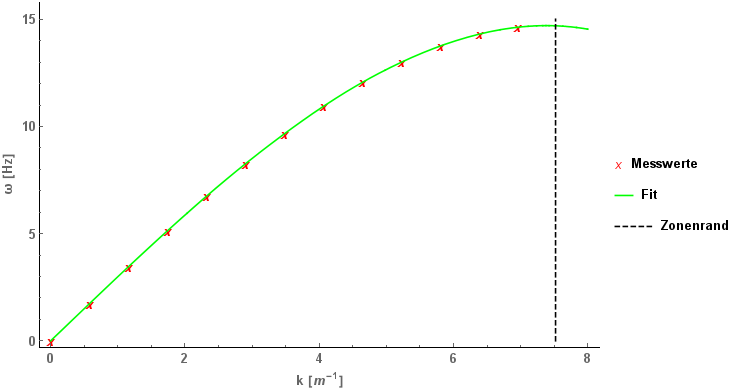
\includegraphics[width=0.75\textwidth]{dispersionsrelationeinatom.png}\\
		\footnotesize\sffamily\textbf{Quelle:} Selbst gezeichnet
	\end{tabular}
	\caption{Dispersionsrelation der einatomigen Kette}
    \label{fig:dispersionsrelationeinatom}
\end{figure}
Die Gitterkonstante $a$ bestimmt man, wie bereits im Abschnitt auf Seite \pageref{eq:einatommodell} zu den Schwingungsmoden des Modellkristalls erklärt, aus:
\begin{equation*}
a=\frac{L}{13}=\frac{\unit[5.43]{m}}{13}=\unit[0.417690]{m}
\end{equation*}
Der systematische Fehler der Gitterkonstante $\sigma_a$ ergibt sich mit Fehlerfortpflanzung zu:
\begin{equation*}
\sigma_a=\frac{\sigma_L}{13}=\unit[0.000385]{m}
\end{equation*}
Also zusammenfassend für die Gitterkonstante $a$:
\begin{equation*}
\boxed{a=\unit[(0.417690 \pm 0.000385)]{m}}
\end{equation*}
Der Zonenrand beträgt $\frac{\pi}{a}=\unit[7.52]{m^{-1}}$ und ist in Abbildung \ref{fig:einatomkettedispersion} eingezeichnet. Der systematische Fehler des Zonenrands $\sigma_z$ bestimmt durch Fehlerfortpflanzung beträgt:
\begin{equation*}
\sigma_z=\frac{\pi}{a^2} \cdot \sigma_a=\frac{\pi}{(\unit[0.417690]{m})^2} \cdot \unit[0.000385]{m}=\unit[0.006933]{m}
\end{equation*}
\subsubsection{Zweiatomige Kette}
Die Dispersionsrelation der zweiatomigen Kette wurde anhand der Daten von Tabellen \ref{tab:akustisch} und \ref{tab:optisch} in Abbildung \ref{fig:dispersionsrelationzweiatom} gezeichnet.
\begin{figure}[H]
	\centering
	\begin{tabular}{@{}r@{}}
		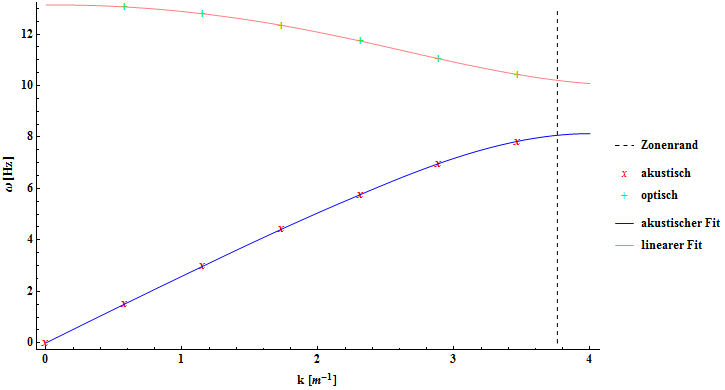
\includegraphics[width=0.75\textwidth]{dispersionsrelationzweiatom.png}\\
		\footnotesize\sffamily\textbf{Quelle:} Selbst gezeichnet
	\end{tabular}
	\caption{Dispersionsrelation der zweiatomigen Kette}
    \label{fig:dispersionsrelationzweiatom}
\end{figure}
Zwecks Fehlerrechnung erweitern wir nun die Tabellen \ref{tab:akustisch} und \ref{tab:optisch} um die Spalten $\sigma_{\overline{f}}$ und $\sigma_{\overline{\omega_n}}$, die wir analog zur Tabelle \ref{tab:einatomigekettemittlere} bestimmen. Der Fehler des Wellenvektors $k_n$ wurde bereits in Tabelle \ref{tab:einatomigekettemittlere} bestimmt und wird hier nicht nochmal aufgelistet.
\begin{table}[H]
\centering
\begin{tabular}{c|c|c|c|c|c}
Mode $n$ & $\overline{f}$ $[\unit[Hz]]$ & $\sigma_{\overline{f}}$ $[\unit[Hz]]$ & $k_n=\frac{n \pi}{L}$ $[\unit[]{m^{-1}}]$ & $\overline{\omega}_n=2 \pi \overline{f}$ $[\unit[]{Hz}]$ & $\sigma_{\overline{\omega_n}}$ $[\unit[]{Hz}]$\\
\hline
1 & 0.240229 & 0.000476 & 0.578562 & 1.509400 & 0.002991\\
2 & 0.476527 & 0.000400 & 1.157120 & 2.994110 & 0.002513\\
3 & 0.705166 & 0.000440 & 1.735690 & 4.430690 & 0.002765\\
4 & 0.919061 & 0.000101 & 2.314250 & 5.774630 & 0.000635\\
5 & 1.111270 & 0.000460 & 2.892810 & 6.982290 & 0.002890\\
6 & 1.248990 & 0.000551 & 3.471370 & 7.847650 & 0.003462
\end{tabular}
\caption{Mittlere Eigenfrequenzen $\overline{f}$, Eigenkreisfrequenzen $\overline{\omega_n}$ des akustischen Astes der zweiatomigen Kette mit Fehlerrechnung}
\label{tab:zweiatomigakustisch}
\end{table}
\begin{table}[H]
\centering
\begin{tabular}{c|c|c|c|c|c}
Mode $n$ & $\overline{f}$ $[\unit[Hz]]$ & $\sigma_{\overline{f}}$ $[\unit[Hz]]$ & $k_n=\frac{n \pi}{L}$ $[\unit[]{m^{-1}}]$ & $\overline{\omega}_n=2 \pi \overline{f}$ $[\unit[]{Hz}]$ & $\sigma_{\overline{\omega_n}}$ $[\unit[]{Hz}]$\\
\hline
6 & 1.66057 & 0.000417 & 3.471370 & 10.433700 & 0.002620\\
5 & 1.75733 & 0.000516 & 2.892810 & 11.041600 & 0.003242\\
4 & 1.86729 & 0.000477 & 2.314250 & 11.732600 & 0.002997\\
3 & 1.96493 & 0.000263 & 1.735690 & 12.346000 & 0.001652\\
2 & 2.03604 & 0.000481 & 1.157120 & 12.792800 & 0.003022\\
1 & 2.07925 & 0.000445 & 0.578562 & 13.064300 & 0.002796
\end{tabular}
\caption{Mittlere Eigenfrequenzen $\overline{f}$, Eigenkreisfrequenzen $\overline{\omega_n}$ des optischen Astes der zweiatomigen Kette mit Fehlerrechnung}
\label{tab:zweiatomigoptisch}
\end{table}
Die Gitterkonstante $a$ der zweiatomigen Kette ist das Doppelte der Gitterkonstante der einatomigen Kette (siehe auch die Gleichung dazu im Abschnitt ''Modellkristall'' auf Seite \pageref{eq:zweiatommodell}):
\begin{equation*}
a=\frac{L}{6.5}=\unit[0.835380]{m}
\end{equation*}
Der systematische Fehler der Gitterkonstante $\sigma_a$ beträgt:
\begin{equation*}
\sigma_a=\frac{\sigma_L}{6.5}=\unit[0.000769]{m}
\end{equation*}
Zusammenfassend beträgt die Gitterkonstante $a$:
\begin{equation*}
\boxed{a=\unit[(0.835380 \pm 0.000769)]{m}}
\end{equation*}
Der Zonenrand beträgt damit $\frac{\pi}{a}=\unit[3.76]{m^{-1}}$ und wurde ebenfalls in Abbildung \ref{fig:dispersionsrelationzweiatom} der Dispersionsrelation eingezeichnet. Der systematische Fehler des Zonenrandes $\sigma_z$ beträgt:
\begin{equation*}
\sigma_z=\frac{\pi}{a^2} \cdot \sigma_a=\frac{\pi}{(\unit[0.835380]{m})^2} \cdot \unit[0.000769]{m}=\unit[0.003462]{m}
\end{equation*}
\subsection{Schallgeschwindigkeit}
Die Schallgeschwindigkeiten für die einatomige $v_{s,1}$ und zweiatomige Kette $v_{s,2}$ lassen sich, laut den Gleichungen \ref{eq:einatomSchallgeschwindigkeit} und \ref{eq:zweiatomschallgeschwindigkeit}, folgendermaßen bestimmen:
\begin{equation*}
v_s=\frac{\omega}{k}
\end{equation*}
Diese Beziehung gilt für Wellenvektore $k$ sehr nahe dem Nullpunkt. Deshalb bestimmen wir die Steigung des linearen Teils der jeweiligen Dispersionskurven, der durch die beiden Punkte $(0,0)$ und $(\omega_1,k_1)$ geht und erhalten:
\begin{align*}
v_{s,1}&=\frac{\omega_1}{k_1}=\frac{\unit[1.739390]{Hz}}{\unit[0.578562]{m^{-1}}}=\unit[3.006402]{\frac{m}{s}}\\
v_{s,2}&=\frac{\omega_1}{k_1}=\frac{\unit[1.509400]{Hz}}{\unit[0.578562]{m^{-1}}}=\unit[2.608882]{\frac{m}{s}}
\end{align*}
Da, wie wir in den vorigen Abschnitten der Auswertung gesehen haben, sowohl die Eigenkreisfrequenzen $\omega$ als auch die Wellenvektoren $k_n$ fehlerbehaftet sind, sind auch die daraus berechneten Schallgeschwindigkeiten fehlerbehaftet. Mit Fehlerfortpflanzung ergibt sich also:
\begin{align*}
\sigma_{v_s}&=\sqrt{\left( \frac{\partial v_s}{\partial \omega} \right)^2 \sigma_{\omega}^2 + \left( \frac{\partial v_s}{\partial k} \right)^2 \sigma_k^2}\\
&=\sqrt{\frac{1}{k^2} \cdot \sigma_{\omega}^2 + \frac{\omega^2}{k^4} \cdot \sigma_k^2}
\end{align*}
Der Fehler der Schallgeschwindigkeit für die einatomige Kette $\sigma_{v_{s,1}}$ beträgt:
\begin{align*}
\sigma_{v_{s,1}}&=\sqrt{\frac{1}{(\unit[0.578562]{m^{-1}})^2} \cdot (\unit[0.003204]{Hz})^2 + \frac{(\unit[1.739390]{Hz})^2}{(\unit[0.578562]{m^{-1}})^4} \cdot (\unit[0.000533]{m^{-1}})^2}\\
&=\unit[0.005792]{\frac{m}{s}}
\end{align*}
Der Fehler der Schallgeschwindigkeit für die zweiatomige Kette $\sigma_{v_{s,2}}$ beträgt:
\begin{align*}
\sigma_{v_{s,2}}&=\sqrt{\frac{1}{(\unit[0.578562]{m^{-1}})^2} \cdot (\unit[0.002991]{Hz})^2 + \frac{(\unit[1.509400]{Hz})^2}{(\unit[0.578562]{m^{-1}})^4} \cdot (\unit[0.000533]{m^{-1}})^2}\\
&=\unit[0.005353]{\frac{m}{s}}
\end{align*}
Zusammenfassend also:
\begin{equation*}
\boxed{v_{s,1}=\unit[(3.006402 \pm 0.005792)]{\frac{m}{s}}}
\end{equation*}
\begin{equation*}
\boxed{v_{s,2}=\unit[(2.608882 \pm 0.005353)]{\frac{m}{s}}}
\end{equation*}
\subsection{Massenverhältnis}
Das Massenverhältnis $\gamma=\frac{M}{m}$ bestimmt sich aus dem Verhältnis der Schallgeschwindigkeiten $v_{s,1}$ und $v_{s,2}$ für $k \rightarrow 0$ (siehe Formeln \ref{eq:einatomSchallgeschwindigkeit} bzw. \ref{eq:zweiatomschallgeschwindigkeit} auf Seiten \pageref{eq:einatomSchallgeschwindigkeit} bzw. \pageref{eq:zweiatomschallgeschwindigkeit}):
\begin{align*}
\frac{v_{s,1}}{v_{s,2}}&=\sqrt{\frac{Da_1^2}{m} \cdot \frac{2(m+M)}{Da_2^2}}\\
&=\sqrt{\frac{D a_1^2}{m} \cdot \frac{2(m+M)}{4Da_1^2}}\\
&=\sqrt{\frac{m+M}{2m}}\\
&=\frac{1}{\sqrt{2}} \cdot \sqrt{1+\frac{M}{m}}\\
\end{align*}
Das Massenverhältnis $\gamma$ beträgt:
\begin{align*}
\gamma&=\frac{M}{m}= 2 \cdot \left(\frac{v_{s,1}}{v_{s,2}}\right)^2-1\\
&=2 \cdot \left(\frac{3.006402}{2.608882}\right)^2-1\\
&=1.655921
\end{align*}
Da $v_{s,1}$ und $v_{s,2}$ fehlerbehaftet sind, so ist auch das Massenverhältnis:
\begin{align*}
\sigma_{\gamma}&=\sqrt{\left( \frac{\partial \gamma}{\partial v_{s,1}} \right)^2 \sigma^2_{v_{s,1}} + \left( \frac{\partial \gamma}{\partial v_{s,2}} \right)^2 \sigma^2_{v_{s,2}}}\\
&=\sqrt{\frac{16 \cdot v^2_{s,1}}{v_{s,2}^4} \cdot \sigma^2_{v_{s,1}}+\frac{16 \cdot v^4_{s,1}}{v_{s,2}^6} \cdot \sigma^2_{v_{s,2}}}\\
&=0.014950
\end{align*}
Mit Fehler beträgt es:
\begin{equation*}
\boxed{\gamma=1.655921 \pm 0.014950}
\end{equation*}
\subsection{Federkonstante der einatomigen Kette}
Es ist die Federkonstante $D$ der einatomigen Kette mit 2 Methoden zu bestimmen:
\subsubsection{Aus der Dispersionsrelation}
Aus Gleichung \ref{eq:dispersionsrelationeinatom} auf Seite \pageref{eq:dispersionsrelationeinatom} gilt für die Dispersionsrelation der einatomigen Kette:
\begin{equation*}
\omega(k)=\sqrt{\frac{4D}{m}} \bigg|\sin{\left( \frac{ka}{2} \right)}\bigg|
\end{equation*}
Durch Umformen ergibt sich die gesuchte Federkonstante $D_1$:
\begin{equation*}
D_1=\frac{m \cdot \omega^2}{4 \sin^2{\left( \frac{ka_1}{2} \right)}}
\end{equation*}
Dabei ist die $a_1$ die Gitterkonstante der einatomigen Kette mit $a_1=\unit[0.41769]{m}$, $m$ die Masse der leichten Gleiter mit $m=\unit[0.504]{kg}$. Für den Wellenvektor $k$ und die Eigenfrequenz $\omega_1$ kann ein beliebiges Wertepaar aus Tabelle \ref{tab:einatomigekettemittlere} herangezogen werden. Wir wählten das erste Paar und erhielten:
\begin{equation*}
D_1=\frac{\unit[0.504]{kg} \cdot (\unit[1.739390]{Hz})^2}{4 \sin^2{\left( \frac{\unit[0.578562]{m^{-1}} \cdot \unit[0.41769]{m}}{2} \right)}}=\unit[26.238000]{\frac{N}{m}}
\end{equation*}
Dabei sind die Kreisfrequenz $\omega(k)$, der Wellenvektor $k$ und die einatomige Gitterkonstante $a_1$ fehlerbehaftet. Auch die daraus berechnete Federkonstante $D_1	$ ist damit fehlerbehaftet (Fehlerfortpflanzung):
\begin{align*}
\sigma_{D_1}&=\sqrt{\left( \frac{\partial D_1}{\partial \omega} \right)^2 \sigma^2_{\omega} + \left( \frac{\partial D_1}{\partial k} \right)^2 \sigma^2_k + \left( \frac{\partial D_1}{\partial a_1} \right)^2 \sigma^2_{a_1}}\\
&=\sqrt{ \left( \frac{m \cdot \omega}{2 \cdot \sin^2{\left( \frac{k a_1}{2} \right)}} \right)^2 \cdot \sigma^2_{\omega} + \left( \frac{a_1 \cdot m \cdot \omega^2}{4 \cdot \tan{\left( \frac{k a_1}{2} \right)} \cdot \sin^2{\left( \frac{k a_1}{2} \right)}} \right)^2 \cdot \sigma^2_k + }\\ 
& \quad \quad \quad \quad \overline{\rule{0pt}{2.5ex} + \left( \frac{k \cdot m \cdot \omega^2}{4 \cdot \tan{\left( \frac{k a_1}{2} \right) \cdot \sin^2{\left( \frac{k a_1}{2} \right)}}} \right)^2 \cdot \sigma^2_{a_1}  }\\
&=\unit[0.056723]{\frac{N}{m}}
\end{align*}
Die Federkonstante $D_1$ samt Fehlergrenzen lautet:
\begin{equation*}
\boxed{D_1=\unit[(26.238000 \pm 0.056273)]{\frac{N}{m}}}
\end{equation*}
\subsubsection{Aus der Schallgeschwindigkeit}
Ein weiterer Weg die Federkonstante $D$ der einatomigen Kette zu bestimmen, ist aus der Schallgeschwindigkeit $v_{s,1}$. Die Schallgeschwindigkeit beträgt laut Gleichung \ref{eq:einatomSchallgeschwindigkeit} auf Seite \pageref{eq:einatomSchallgeschwindigkeit}:
\begin{equation*}
v_{s,1}=\sqrt{\frac{D a_1^2}{m}}
\end{equation*}
Also erhält man daraus die Federkonstante $D_2$:
\begin{equation*}
D_2=\frac{m \cdot v_{s,1}^2}{a_1^2}
\end{equation*}
Wir setzen darin den 1. Wertepaar $(\omega_1, k_1)$ ein (denn da liegt $k$ sehr nahe dem Nullpunkt):
\begin{equation*}
D_2=\frac{\unit[0.504]{kg} \cdot (\unit[3.006402]{\frac{m}{s}})^2}{(\unit[0.41769]{m})^2}=\unit[26.1106]{\frac{N}{m}}
\end{equation*}
Weil die Schallgeschwindigkeit $v_{s,1}$ und die Gitterkonstante $a_1$ fehlerbehaftet sind, ist auch die davon abhängige Federkonstante $D_2$ mit dem Fehler nach dem Fehlerfortpflanzungsgesetz fehlerbehaftet:
\begin{align*}
\sigma_{D_2}&=\sqrt{ \left( \frac{\partial D_2}{\partial v_{s,1}} \right)^2 \sigma^2_{v_{s,1}} + \left( \frac{\partial D_2}{\partial a_1} \right)^2 \sigma^2_{a_1}}\\
&=\sqrt{ \left( \frac{2 \cdot m \cdot v_{s,1}}{a^2_1} \right)^2 \sigma^2_{v_{s,1}} + \left( \frac{2 \cdot m \cdot v^2_{s,1}}{a_1^3} \right)^2 \sigma^2_{a_1}}\\
&=\unit[0.063897]{\frac{N}{m}}
\end{align*}
Zusammenfassend für die Federkonstante $D_2$ haben wir:
\begin{equation*}
\boxed{D_2=\unit[(26.110600 \pm 0.063897)]{\frac{N}{m}}}
\end{equation*}
\subsection{Federkonstante der zweiatomigen Kette}
Auch für die zweiatomige Kette soll die Federkonstante $D$ aus der Dispersionsrelation aus Gleichung \ref{eq:dispersionsrelationzweiatom} auf Seite \pageref{eq:dispersionsrelationzweiatom} bestimmt werden. Wir nehmen den akustischen Ast:
\begin{equation*}
\omega(k)^2=D \left( \frac{1}{m} + \frac{1}{M} \right) - D \sqrt{\left( \frac{1}{m} + \frac{1}{M} \right)^2 - \frac{4}{m M} \sin^2{\left( \frac{ka_2}{2} \right)}}
\end{equation*}
Auflösen nach der gesuchten $D$:
\begin{equation*}
D_3=\frac{\omega^2}{\left( \frac{1}{m} + \frac{1}{M} \right) - \sqrt{\left( \frac{1}{m} + \frac{1}{M} \right)^2 - \frac{4}{mM} \sin^2{\left( \frac{ka_2}{2} \right)}}}
\end{equation*}
Die unbekannte Masse $M$ des schweren Gleiters kann aus dem zuvor bestimmten Massenverhältnis $\gamma=\frac{M}{m}$ und aus der bekannten Masse des leichten Gleiters $m=\unit[0.504]{kg}$ berechnet werden:
\begin{equation*}
M=\gamma \cdot m = 1.655921 \cdot \unit[0.504]{kg}=\unit[0.834584]{kg}
\end{equation*}
Da das Massenverhältnis fehlerbehaftet war, muss dies bei der Masse des schweren Gleiters $M$ ebenfalls berücksichtigt werden (Fehlerfortpflanzung):
\begin{equation*}
\sigma_M=m \cdot \sigma_{\gamma}=\unit[0.504]{kg} \cdot 0.014950=\unit[0.007535]{kg}
\end{equation*}
Wir wählten dann willkürlich das erste Wertepaar $(\omega_1,k_1)$ aus Tabelle \ref{tab:akustisch} auf Seite \pageref{tab:akustisch} und erhielten:
\begin{align*}
D_3&=\frac{(\unit[1.509400]{Hz})^2}{\left( \frac{1}{\unit[0.504]{kg}} + \frac{1}{\unit[0.834584]{kg}} \right) - \sqrt{\left( \frac{1}{\unit[0.504]{kg}} + \frac{1}{\unit[0.834584]{kg}} \right)^2 - \frac{4}{\unit[0.504]{kg} \cdot \unit[0.834584]{kg}} \cdot \sin^2{\left( \frac{\unit[0.578562]{m^{-1}} \cdot \unit[0.83538]{m}}{2} \right)}}}\\
&=\unit[26.2619]{\frac{N}{m}}
\end{align*}
Der Fehler $\sigma_{D_3}$ der bestimmten Federkonstante $D_3$ entsteht aus dem Fortpflanzung der Fehler der abhängigen Größen $\omega$, $M$, $k$ und $a_2$:
\begin{align*}
\sigma_{D_3}&=\sqrt{\left( \frac{\partial D_3}{\partial \omega} \right)^2 \cdot \sigma^2_{\omega} + \left( \frac{\partial D_3}{\partial M} \right)^2 \sigma^2_M + \left( \frac{\partial D_3}{\partial k} \right)^2 \sigma^2_k + \left( \frac{\partial D_3}{\partial a_2} \right)^2 \sigma^2_{a_2}}\\
\end{align*}
Dabei gilt:
\begin{align*}
\frac{\partial D_3}{\partial \omega}&=\frac{2 \omega}{\frac{1}{m}+\frac{1}{M}-\sqrt{\left( \frac{1}{m} + \frac{1}{M} \right)^2 - \frac{4 \sin^2{\left( \frac{a_2 k}{2} \right)}}{m \cdot M}}}\\
\frac{\partial D_3}{\partial M}&=-\frac{\omega^2 \left( -\frac{1}{M^2} + \frac{m+M-2 \cdot M \cdot \sin{\left( \frac{a_2 k}{2} \right)}}{M^2 \sqrt{(m+M)^2-4mM \sin{\left( \frac{a_2 k}{2} \right)}}} \right)}{\left( \frac{1}{m} + \frac{1}{M} - \sqrt{\frac{(m+M)^2- 4 \cdot m \cdot M \sin{\left( \frac{a_2 k}{2} \right)}}{m^2 M^2}} \right)^2}\\
\frac{\partial D_3}{\partial k}&=-\frac{a_2 \cdot m \cdot M \cdot \omega^2 \cos{\left( \frac{k a_2}{2} \right)}}{\sqrt{\frac{(m + M)^2-4 m M \sin{\left( \frac{a_2 k}{2} \right)}}{m^2 M^2}} \left( M-m\left( -1 + \sqrt{\frac{(m+M)^2-4mM \sin{\left( \frac{k a_2}{2} \right)}}{m^2}} \right) \right)^2}\\
\frac{\partial D_3}{\partial a_2}&=-\frac{k \cdot m \cdot M \cdot \omega^2 \cdot \cos{\left( \frac{k a_2}{2} \right)}}{\sqrt{\frac{(m+M)^2-4mM \sin{\left( \frac{k a_2}{2} \right)}}{m^2 M^2}} \left( M-m\left( -1 + \sqrt{\frac{(m+M)^2-4mM \sin{\left( \frac{k a_2}{2} \right)}}{m^2}} \right) \right)^2}
\end{align*}
Nach Einsetzen der Werte in die Gleichung des Fehlers $\sigma_{D_3}$ erhält man:
\begin{equation*}
\sigma_{D_3}=\unit[0.042775]{\frac{N}{m}}
\end{equation*}
Damit beträgt die Federkonstante $D_3$ mit Fehlergrenzen:
\begin{equation*}
\boxed{D_3=\unit[(26.261900 \pm 0.042775)]{\frac{N}{m}}}
\end{equation*}
\subsection{Amplitudenverhältnisse}
Es sind nun die Amplitudenverhältnisse $\frac{s_{0,m}}{s_{0,M}}$ der Auslenkungen der leichten und schweren Gleiter zu bestimmen.\\ \\
Da die leichten und schweren Massen sich in unterschiedlichen Positionen befinden und die Amplituden an diesen Stellen gemessen wurden, müssen sie korrigiert werden, um die Positionsunabhängigkeit des Amplitudenverhältnises zu erreichen. Dabei gilt für die Amplitude einer Schwingung am Ort $x$:
\begin{equation*}
s_0(x)=s_0 \sin{(kx)}
\end{equation*}
wobei $s_0$ die maximale Amplitude, $k=\frac{n \pi}{13 a_2}$ der Wellenvektor und $x$ die Position der Gleiter in der Kette sind. Weiterhin gilt $x=\frac{a_2}{2} j$ mit $a_2$ die Gitterkonstante.\\ \\
Der leichte Gleiter befand sich bei uns in Position 6, der schwere in Position 5. Das korrigierte Amplitudenverhältnis zweier benachbarter Gleiter beträgt also:
\begin{equation*}
\frac{s_{0,m}(j)}{s_{0,M}(j-1)}=\frac{1}{a} \cdot \frac{s_{0,m}^{Punkt}}{s_{0,M}^{Punkt}} \quad \quad \quad \text{mit} \quad a=\bigg| \frac{\sin{\left( \frac{n \pi}{13} j \right)}}{\sin{ \left( \frac{n \pi}{13} (j-1) \right) }} \bigg|
\end{equation*}
$a$ ist der Korrekturfaktor des Amplitudenverhältnisses. Durch obige Formel könnten wir die Amplitudenverhältnisse berechnen. Wir bildeten für jeden Gleiter in einer Mode die Mittelwerte ihrer jeweiligen Amplituden, bestimmten den modenabhängigen Korrekturfaktor und anschließend daraus das Amplitudenverhältnis dieser Gleiter für die Mode.\\ \\
Jede gemessene Amplitude ist mit einem systematischen Fehler aufgrund der Apparatur behaftet, den wir hier nicht berücksichtigen werden. Die Mittelwerte der Amplituden $\overline{s_{0,m}^{Punkt}}$, $\overline{s_{0,M}^{Punkt}}$ sind mit statistischem Fehler $\sigma_{s(6)}$ bzw. $\sigma_{s(5)}$ aufgrund der Standardabweichung behaftet.\\ \\
Dadurch ist das Amplitudenverhältnis auch mit einem Fehler $\sigma_A$ behaftet (Fehlerfortpflanzung):
\begin{align*}
\sigma_A&=\sqrt{\left( \frac{\partial A}{\partial s_{0,m}^{Punkt}} \right)^2 \cdot \sigma^2_{s(6)} + \left( \frac{\partial A}{\partial s_{0,M}^{Punkt}} \right)^2 \cdot \sigma^2_{s(5)}}\\
&=\sqrt{\frac{1}{a^2 \cdot s_{0,M}^2} \cdot \sigma^2_{s_{0,m}} + \frac{s_{0,m}^2}{a^2 \cdot s^4_{0,M}} \cdot \sigma^2_{s_{0,M}}}
\end{align*}
Diese Ergebnisse für die akustischen und optischen Moden finden sich jeweils in Tabellen \ref{tab:amplitudenverhaeltnisseAkustisch} und \ref{tab:amplitudenverhaeltnisseOptisch}.
\begin{table}[H]
\centering
\renewcommand{\tabcolsep}{1pt}
\begin{tabular}{@{}c|c|c|c|c|c|c|c@{}}
Mode $n$ & $\overline{s_{0,m}^{Punkt}(6)}$ $[\unit[]{mm}]$ & $\sigma_{s(6)}$ $[\unit[]{mm}]$ & $\overline{s_{0,M}^{Punkt}(5)}$ $[\unit[]{mm}]$ & $\sigma_{s(5)}$ $[\unit[]{mm}]$ & $a$ & $\frac{1}{a} \cdot \frac{\overline{s_{0,m}^{Punkt}(6)}}{\overline{s_{0,M}^{Punkt}(5)}}$ & $\sigma_A$\\
\hline
1 & 63.632200 & 0.187230 & 62.182200 & 0.210149 & 1.061700 & 0.963849 & 0.004319\\
2 & 48.729400 & 0.134083 & 142.550000 & 0.178939 & 0.360892 & 0.947212 & 0.002865\\
3 & 99.888900 & 0.189871 & 55.368500 & 0.110198 & 2.011990 & 0.896661 & 0.002468\\
4 & 43.016700 & 0.176402 & 111.831000 & 0.187229 & 0.468136 & 0.821678 & 0.003640\\
5 & 45.910000 & 0.092146 & 22.045400 & 0.055099 & 3.438910 & 0.605576 & 0.011023\\
6 & 17.547700 & 0.088202 & 74.990500 & 0.192230 & 0.805754 & 0.290410 & 0.001639\\
\end{tabular}
\caption{Amplitudenverhältnisse für die akustischen Moden}
\label{tab:amplitudenverhaeltnisseAkustisch}
\end{table}
\begin{table}[H]
\centering
\renewcommand{\tabcolsep}{1pt}
\begin{tabular}{@{}c|c|c|c|c|c|c|c@{}}
Mode $n$ & $\overline{s_{0,m}^{Punkt}(6)}$ $[\unit[]{mm}]$ & $\sigma_{s(6)}$ $[\unit[]{mm}]$ & $\overline{s_{0,M}^{Punkt}(5)}$ $[\unit[]{mm}]$ & $\sigma_{s(5)}$ $[\unit[]{mm}]$ & $a$ & $\frac{1}{a} \cdot \frac{\overline{s_{0,m}^{Punkt}(6)}}{\overline{s_{0,M}^{Punkt}(5)}}$ & $\sigma_A$\\
\hline
1 & 10.418500 & 0.147073 & 6.108800 & 0.141149 & 1.061700 & 1.606380 & 0.043496\\
2 & 5.954400 & 0.090064 & 9.230330 & 0.136884 & 0.360892 & 1.787490 & 0.037864\\
3 & 30.778900 & 0.122238 & 9.465280 & 0.111055 & 2.011990 & 1.616200 & 0.020028\\
4 & 16.138000 & 0.103081 & 19.393800 & 0.147557 & 0.468136 & 1.777520 & 0.017658\\
5 & 28.838900 & 0.127742 & 3.568290 & 0.266583 & 3.438910 & 2.350160 & 0.175886\\
6 & 16.413200 & 0.319725 & 4.323150 & 0.141820 & 0.805754 & 4.711840 & 0.179769\\
\end{tabular}
\caption{Amplitudenverhältnisse für die optischen Moden}
\label{tab:amplitudenverhaeltnisseOptisch}
\end{table}
Die bestimmten Amplitudenverhältnisse waren anschließend gegen $k_n$ aufzutragen (Abbildung \ref{fig:amplitudenverhaeltnisse}). Da die leichten und schweren Massen im optischen Ast gegenphasig schwingen, ist das Amplitudenverhältnis der Gleiter negativ. Die obigen Tabellen \ref{tab:amplitudenverhaeltnisseAkustisch} und \ref{tab:amplitudenverhaeltnisseOptisch} zeigen nur die Beträge der Amplitudenverhältnisse.
\begin{figure}[H]
	\centering
	\begin{tabular}{@{}r@{}}
		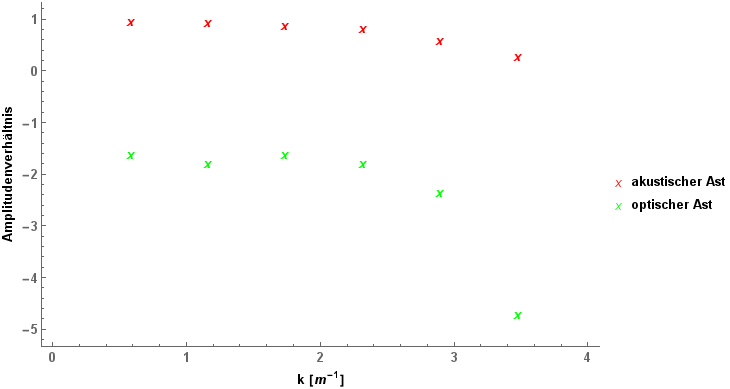
\includegraphics[width=0.75\textwidth]{amplitudenverhaeltnis.png}\\
		\footnotesize\sffamily\textbf{Quelle:} Selbst gezeichnet
	\end{tabular}
	\caption{Amplitudenverhältnisse}
    \label{fig:amplitudenverhaeltnisse}
\end{figure}
\section{Diskussion der Ergebnisse}
Wir bestimmten und zeichneten die Dispersionsrelationen der einatomigen und zweiatomigen Ketten aus den gemessenen Eigenfrequenzen und stellten fest, dass diese sehr gut mit der in der Vorbereitung aus dem mathematischen Modell gezeichneten Dispersionsrelation übereinstimmen. Auch die Fehler der Eigenkreisfrequenzen $\omega_n$ und der Wellenvektoren $k_n$ waren sehr klein. Im Anschluss wurden auch die Gitterkonstanten der linearen Ketten berechnet.\\ \\
Danach wurden die Schallgeschwindigkeiten für die einatomige und zweiatomige Kette bestimmt. Diese waren aufgrund der sehr kleinen Fehler sehr gut. Das Gleiche lässt sich auch für das bestimmte Massenverhältnis sagen.\\ \\
Die Federkonstanten wurden nach 3 Methoden berechnet: aus der einatomigen Kette anhand ihrer Dispersionsrelation und Schallgeschwindigkeit und aus der zweiatomigen Kette anhand ihrer Dispersionsrelation. Wir erhielten jeweils:
\begin{equation*}
\boxed{D_1=\unit[(26.238000 \pm 0.056273)]{\frac{N}{m}}} \quad \boxed{D_2=\unit[(26.110600 \pm 0.063897)]{\frac{N}{m}}}
\end{equation*}
\begin{equation*}
\boxed{D_3=\unit[(26.261900 \pm 0.042775)]{\frac{N}{m}}}
\end{equation*}
Diese Werte stimmen unter Berücksichtigung der Fehlergrenzen sehr gut miteinander überein.\\ \\
Anschließend wurden die Amplitudenverhältnisse zwei benachbarter Gleiter bestimmt. Auch hier waren die Ergebnisse zufriedenstellend. So konnte man für den akustischen Ast beobachten, wie am Anfang das Amplitudenverhältnis fast 1 war, also die leichte und schwere Masse gleich große Auslenkungen hatten. Für größere Wellenvektoren nahm das Verhältnis ab und ging gegen 0, d.h. die leichten Massen ruhten. Im optischen Ast war das Verhältnis für kleine Wellenvektoren $k$ relativ konstant, fallte jedoch am Ende in der Nähe der 1. Brioullin Zone stark ab, d.h. die schweren Massen ruhten.\\ \\
Wir können zusammenfassend behaupten, dass die mathematischen Beschreibungen der linearen einatomigen und zweiatomigen Kette mit ihren Vereinfachungen das reale Verhalten solcher Ketten sehr gut modellieren können. Jedoch konnte in diesem Versuch keine Verknüpfung des realen Festkörpers zum Modell der linearen Kette aufgezeigt werden.
\bibliographystyle{acm}
\bibliography{literatur}

\end{document}